\subsubsection{Dataset Collection}

\noindent Our dataset acquisition process involved the following steps:

\begin{enumerate}
    \item \textbf{Public Datasets:} We sourced a significant portion of our dataset from publicly available deepfake and real image datasets. These datasets were chosen for their variety and relevance to our detection task.

    \item \textbf{Video Conversion:} To include videos in our dataset, we first converted them into individual frames (images) to facilitate compatibility with the vision transformer architecture. This step involved extracting frames at a consistent frame rate from each video, resulting in a sequence of images for each video.

    \item \textbf{Frame Selection:} To avoid redundancy and maintain dataset balance, we carefully selected frames from videos to represent various stages of manipulation, expressions, poses, and lighting conditions.

    \item \textbf{Annotation and Labeling:} Each image was labeled as either "real" or "deepfake." Annotations were done manually to ensure accurate labeling for training and evaluation.
\end{enumerate}
% \begin{figure}[h]
%     \centering
%     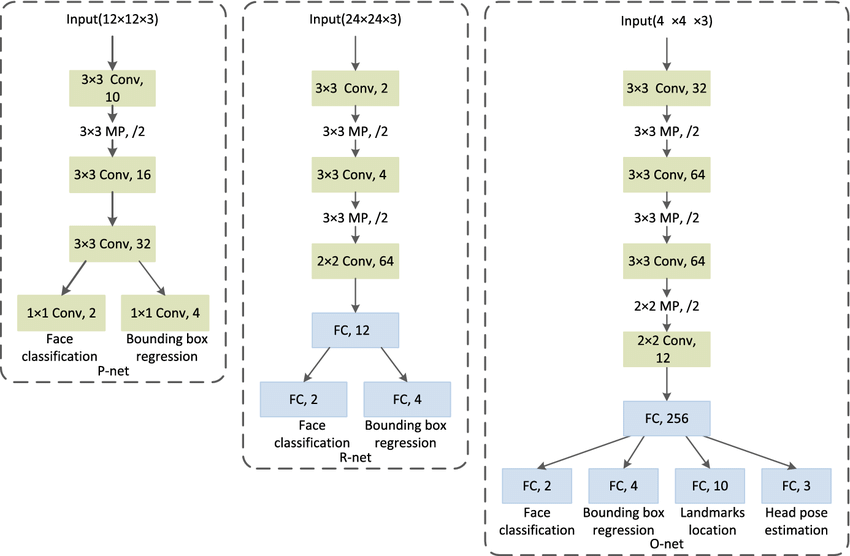
\includegraphics[width= 5in ]{img/MTCNN.png}
%     \caption{MTCNN Architecture}
% \end{figure}